% How VPO works — data-flow figure for the README.
% Build:  pdflatex how_vpo_works.tex
%         pdftoppm -png -r 200 -singlefile how_vpo_works.pdf how_vpo_works
\documentclass[border=8pt]{standalone}
\usepackage{tikz}
\usetikzlibrary{arrows.meta, positioning}

\definecolor{vpoblue}{HTML}{1F4E79}
\definecolor{vpofill}{HTML}{EAF1FB}
\definecolor{taskfill}{HTML}{FBEFE3}
\definecolor{taskline}{HTML}{B5712A}
\definecolor{neutralfill}{HTML}{F2F2F2}

\begin{document}
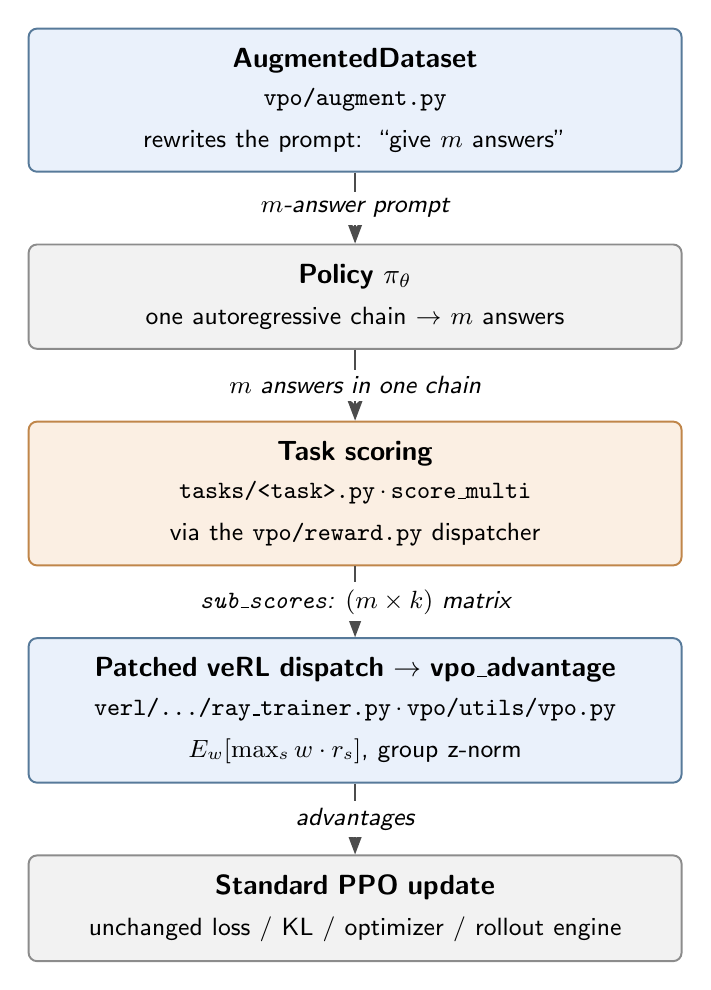
\begin{tikzpicture}[
  font=\sffamily,
  node distance=9mm,
  box/.style   ={rounded corners=3pt, text width=78mm, align=center,
                 inner sep=7pt, line width=0.7pt},
  vpo/.style   ={box, draw=vpoblue!75, fill=vpofill},
  task/.style  ={box, draw=taskline!85, fill=taskfill},
  neu/.style   ={box, draw=black!45, fill=neutralfill},
  flow/.style  ={-{Stealth[length=3mm]}, line width=1pt, draw=black!70},
  lab/.style   ={font=\sffamily\small\itshape, fill=white, inner sep=2.5pt},
]

\node[vpo]  (aug)   {\textbf{AugmentedDataset}\\[2pt]
                     \texttt{\small vpo/augment.py}\\[3pt]
                     \small rewrites the prompt: ``give $m$ answers''};
\node[neu, below=of aug]   (pol)
                    {\textbf{Policy} $\pi_\theta$\\[3pt]
                     \small one autoregressive chain $\rightarrow$ $m$ answers};
\node[task, below=of pol]  (score)
                    {\textbf{Task scoring}\\[2pt]
                     \texttt{\small tasks/<task>.py\,$\cdot$\,score\_multi}\\[3pt]
                     \small via the \texttt{\small vpo/reward.py} dispatcher};
\node[vpo, below=of score] (adv)
                    {\textbf{Patched veRL dispatch} $\rightarrow$ \textbf{vpo\_advantage}\\[2pt]
                     \texttt{\small verl/.../ray\_trainer.py\,$\cdot$\,vpo/utils/vpo.py}\\[3pt]
                     \small $E_{w}\!\left[\max_{s} w \cdot r_s\right]$, group z\hbox{-}norm};
\node[neu, below=of adv]   (ppo)
                    {\textbf{Standard PPO update}\\[3pt]
                     \small unchanged loss / KL / optimizer / rollout engine};

\draw[flow] (aug)   -- (pol)   node[lab, midway] {$m$-answer prompt};
\draw[flow] (pol)   -- (score) node[lab, midway] {$m$ answers in one chain};
\draw[flow] (score) -- (adv)   node[lab, midway] {\texttt{sub\_scores}: $(m \times k)$ matrix};
\draw[flow] (adv)   -- (ppo)   node[lab, midway] {advantages};

\end{tikzpicture}
\end{document}
